\documentclass[12pt, a4paper]{article}

% ── Packages ──────────────────────────────────────────────────────────
\usepackage[margin=2.5cm]{geometry}
\usepackage{graphicx}
\usepackage{amsmath}
\usepackage{booktabs}
\usepackage{hyperref}
\usepackage{float}
\usepackage{caption}
\usepackage[backend=bibtex, style=ieee]{biblatex}
\addbibresource{refs.bib}

% Figures live in one place only: the directory the pipeline writes them to.
\graphicspath{{../results/figures/}}

% Every number in this report is a macro defined in generated.tex, which is
% written by scripts/update_report.py from results/metrics/*.json. No figure is
% typed into the prose. Regenerate with:
%     python scripts/update_report.py
% ─────────────────────────────────────────────────────────────────────
% GENERATED FILE — do not edit.
% Written by scripts/update_report.py from results/metrics/*.json.
% Every number in main.tex comes from here, so the report cannot drift
% from the run that produced it.
% ─────────────────────────────────────────────────────────────────────

\newcommand{\runDate}{2026-09-22}
\newcommand{\runSeed}{1337}
\newcommand{\runDevice}{cuda}
\newcommand{\nTest}{50}
\newcommand{\countTol}{3}
\newcommand{\trainEpochs}{10}
\newcommand{\trainImgsz}{640}
\newcommand{\trainBatch}{16}

\newcommand{\WsIoU}{0.065}
\newcommand{\WsAcc}{28}
\newcommand{\WsMae}{8.66}
\newcommand{\WsMs}{13}
\newcommand{\WsPred}{4.2}
\newcommand{\KmIoU}{0.252}
\newcommand{\KmAcc}{0}
\newcommand{\KmMae}{114.86}
\newcommand{\KmMs}{88}
\newcommand{\KmPred}{127.5}
\newcommand{\YoIoU}{0.429}
\newcommand{\YoAcc}{52}
\newcommand{\YoMae}{4.28}
\newcommand{\YoMs}{26}
\newcommand{\YoPred}{9.1}
\newcommand{\HyIoU}{0.456}
\newcommand{\HyAcc}{64}
\newcommand{\HyMae}{3.30}
\newcommand{\HyMs}{62}
\newcommand{\HyPred}{11.4}
\newcommand{\gtCount}{12.6}
\newcommand{\gateFired}{41}
\newcommand{\blendApplied}{4}
\newcommand{\gainTotal}{49}
\newcommand{\gainRelaxed}{46}
\newcommand{\gainWatershed}{3}
\newcommand{\watershedShare}{6}
\newcommand{\accGain}{12}
\newcommand{\maeDrop}{23}

\newcommand{\resultsTable}{%
\begin{table}[H]
\centering
\caption{All four methods evaluated in a single run on the same 50 held-out test images, with identical metric definitions, on one device (\texttt{cuda}, seed 1337, \runDate). Instance IoU is class-agnostic under greedy one-to-one matching; unmatched ground-truth instances score zero and are included in the mean. Latency is a median with an interquartile range.}
\label{tab:results}
\begin{tabular}{llrrrr}
\toprule
Method & Type & Mean IoU & Count acc.\ ($\pm$3) & MAE & Median (ms) \\
\midrule
Watershed & Classical & 0.065 & 28\% & 8.66 & 13 \\
KMeans ($k{=}5$) & Classical & 0.252 & 0\% & 114.86 & 88 \\
YOLOv8s-seg (fine-tuned) & Deep learning & 0.429 & 52\% & 4.28 & 26 \\
\textbf{Hybrid (density-aware)} & Hybrid & \textbf{0.456} & \textbf{64\%} & \textbf{3.30} & 62 \\
\bottomrule
\end{tabular}
\end{table}
}

\newcommand{\ablationTable}{%
\begin{table}[H]
\centering
\caption{Decomposition of the hybrid's improvement over YOLOv8s-seg alone. The density-gated relaxed detector pass accounts for almost all of it; the watershed cross-check contributes \watershedShare\% while firing on \blendApplied\ of \nTest\ images.}
\label{tab:ablation}
\begin{tabular}{lrrr}
\toprule
Subset & Images & MAE (YOLO $\rightarrow$ hybrid) & Objects recovered \\
\midrule
Gate fired & 41 & 4.66 $\rightarrow$ 3.46 & 49 \\
Gate did not fire & 9 & 2.56 $\rightarrow$ 2.56 & 0 \\
\midrule
\textit{of which:} relaxed pass & -- & -- & \gainRelaxed \\
\textit{of which:} watershed & \blendApplied & -- & \gainWatershed \\
\midrule
\textbf{Total} & \textbf{\nTest} & \textbf{\YoMae\ $\rightarrow$ \HyMae} & \textbf{\gainTotal} \\
\bottomrule
\end{tabular}
\end{table}
}



\hypersetup{
    colorlinks=true,
    linkcolor=blue,
    citecolor=blue,
    urlcolor=blue
}

% ══════════════════════════════════════════════════════════════════════
\begin{document}

% ── 1. Title Page ─────────────────────────────────────────────────────
\begin{titlepage}
\centering
\vspace*{4cm}
{\Huge\bfseries High-Density Object Segmentation\\[0.4cm]
 Baseline, Deep Learning \& Hybrid Study\par}
\vspace{1.5cm}
{\Large Pranay Sarkar\par}
\vspace{0.5cm}
{\large May 2026\par}
\vfill
{\normalsize Classical baselines · Fine-tuned YOLOv8s-seg · Density-aware hybrid}
\vspace{0.4cm}
{\small All results from a single evaluation run — \runDate, seed \runSeed, \nTest\ held-out test images}
\end{titlepage}

% ── 2. Abstract ───────────────────────────────────────────────────────
\begin{abstract}
Segmenting and counting individual object instances in densely crowded images
remains a difficult problem in computer vision.  This study compares two
classical methods --- Watershed and KMeans colour clustering --- against a
fine-tuned YOLOv8s instance-segmentation model and a density-aware hybrid, on
the subset of COCO val2017 containing 5--50 non-crowd objects per image.
All four methods are evaluated in a \emph{single} run on the same \nTest\
held-out images under identical, class-agnostic metric definitions.
Watershed systematically under-counts (\WsPred\ predicted against \gtCount\
true objects, MAE~\WsMae, \WsAcc\% count accuracy) and KMeans catastrophically
over-counts (\KmPred\ regions, MAE~\KmMae, \KmAcc\% accuracy) --- both for
structural reasons rather than for want of tuning.  Fine-tuning YOLOv8s-seg
for \trainEpochs\ epochs reaches \YoAcc\% accuracy at \YoIoU\ mean IoU.  The
hybrid, which detects crowding from Canny edge density before relaxing the
detector and cross-checking against Watershed, reaches \HyAcc\% accuracy
(\accGain\ points above the detector alone) and reduces counting MAE by
\maeDrop\%.  An ablation attributes \gainRelaxed\ of the \gainTotal\ objects
of recovered counting error to the relaxed detector pass and only
\gainWatershed\ to the Watershed cross-check, so the method is more accurately
characterised as density-aware two-pass detection with a marginal classical
correction than as an equal coupling of the two paradigms.  We also show that
mean IoU alone is insufficient on this task: KMeans attains \KmIoU\ IoU while
getting the object count right on none of the \nTest\ images, because it emits
roughly ten times more regions than there are objects.
\end{abstract}

\tableofcontents
\newpage

% ── 3. Introduction ──────────────────────────────────────────────────
\section{Introduction}

Instance segmentation — the task of detecting every object in an image and
delineating its precise pixel-level boundary — is one of the most challenging
problems in computer vision.  The difficulty increases dramatically in
\emph{high-density} scenes where dozens of objects overlap, occlude one
another, and vary widely in scale.

Dense object segmentation has numerous real-world applications:
\begin{itemize}
    \item \textbf{Retail shelf analysis}: automatically counting products on
          crowded supermarket shelves for inventory management.
    \item \textbf{Crowd analysis}: estimating crowd density and tracking
          individuals in surveillance footage.
    \item \textbf{Biological cell imaging}: counting and segmenting cells in
          microscopy images where cells frequently touch or overlap.
\end{itemize}

The fundamental obstacles in dense segmentation are twofold.  First,
\textbf{occlusion} causes object boundaries to be partially or fully hidden,
making it impossible to recover shape information from pixel intensities
alone.  Second, \textbf{scale variation} means that objects in the same image
can range from a few pixels to thousands, rendering fixed-scale processing
pipelines inadequate.

The objective of this project is to establish a rigorous baseline by applying
classical segmentation methods to a curated dense subset of the COCO
benchmark, quantifying their limitations, and thereby motivating the adoption
of deep-learning methods in Phase~2.

% ── 4. Literature Review ─────────────────────────────────────────────
\section{Literature Review}

\subsection{Classical Image Segmentation}
Graph-based segmentation methods treat each pixel as a node in a graph and
define edge weights based on visual similarity.  Felzenszwalb and
Huttenlocher~\cite{felzenszwalb2004} proposed an efficient algorithm with
$O(n \log n)$ complexity that merges regions greedily when the inter-region
difference is smaller than the intra-region variation.  While elegant,
graph-based methods struggle in dense scenes because the visual similarity
between adjacent objects of the same category produces weak edge weights,
leading to under-segmentation.

\subsection{Watershed Algorithm}
The Watershed algorithm, formalised by Vincent and
Soille~\cite{vincent1991watershed}, treats the greyscale image as a
topographic surface.  ``Water'' fills local minima (catchment basins) and
rises until basins merge; the lines where they meet form segmentation
boundaries.  Pre-processing with a distance transform converts the binary
foreground into a height map so that object centres become peaks and touching
boundaries become valleys.  However, when objects are in physical contact —
as is common in crowded images — the valley between them vanishes, causing
over-merging.

\subsection{COCO Dataset}
The Microsoft COCO (Common Objects in Context) dataset~\cite{lin2014coco} is
the de facto standard benchmark for object detection and instance
segmentation.  It contains over 200,000 labelled images across 80 object
categories, with polygon-level annotations for each instance.  The
validation split (val2017) used in this study contains 5,000 images and
36,335 annotations.  COCO's emphasis on ``objects in context'' — natural
scenes with multiple, often overlapping objects — makes it ideal for
studying dense segmentation.

\subsection{YOLO Family and YOLOv8}
The You Only Look Once (YOLO) family, introduced by Redmon
et~al.~\cite{redmon2016yolo}, revolutionised real-time object detection by
framing detection as a single regression problem over a spatial grid, avoiding
the two-stage region proposal bottleneck.  Each grid cell predicts bounding
boxes, confidence scores, and class probabilities in a single forward pass.
YOLOv8~\cite{jocher2023yolov8}, developed by Ultralytics, extends the YOLO
paradigm with an anchor-free detection head, improved CSPDarknet backbone, and
a prototype-based instance segmentation head.  It achieves state-of-the-art
speed-accuracy trade-offs on COCO, surpassing prior YOLO versions and closing
the gap with two-stage methods on the mAP50-95 metric.

\subsection{Instance Segmentation and Mask R-CNN}
He et~al.~\cite{he2017maskrcnn} introduced Mask~R-CNN, a two-stage detector
that extends Faster~R-CNN with a parallel branch for predicting binary
instance masks.  The key insight is that instance masks can be decoded from
region-of-interest (RoI) aligned features, decoupling class prediction from
mask generation.  Two-stage detectors generally achieve higher mask quality
than single-stage methods (e.g.\ YOLO) at the cost of higher inference
latency, making single-stage approaches preferable for real-time dense-scene
applications.

\subsection{Benchmarking with COCO mAP}
The COCO benchmark evaluates instance segmentation using mean Average
Precision (mAP), computed by averaging the AP over all 80 categories and over
IoU thresholds from 0.50 to 0.95 in steps of 0.05 (mAP50-95).  This metric
is stricter than the PASCAL VOC mAP50 standard and rewards precise
localisation.  For dense scenes, mAP50 is often reported separately as a
measure of detection recall at relaxed localisation.

\subsection{Gap Addressed by This Project}
While individual classical methods have been evaluated on simple
benchmarks, no single study systematically compares Watershed and colour
clustering on a density-stratified subset of a modern benchmark like COCO,
and then directly compares them to a fine-tuned YOLOv8 model on the same
images.  This project fills that gap by providing a controlled ablation study
that quantifies exactly \emph{where} and \emph{why} classical methods fail
and by how much deep learning improves over them on the dense subset.

% ── 5. Dataset & EDA ────────────────────────────────────────────────
\section{Dataset \& Exploratory Data Analysis}

\subsection{Dataset Overview}

\begin{table}[H]
\centering
\caption{COCO val2017 summary statistics.}
\label{tab:dataset}
\begin{tabular}{lr}
\toprule
\textbf{Metric}             & \textbf{Value} \\
\midrule
Total images                & 5,000          \\
Total annotations (non-crowd) & 36,335       \\
Unique categories           & 80             \\
Avg objects / image         & 7.27           \\
Min objects / image         & 0              \\
Max objects / image         & 62             \\
Dense images (5–50 obj.)    & 2,463          \\
\bottomrule
\end{tabular}
\end{table}

\subsection{Object Density Distribution}

Figure~\ref{fig:density} shows the distribution of object counts per image.
The vast majority of images contain fewer than 15~objects, with a sharp drop
in frequency beyond 20.  Only 60~images (1.2\%) fall in the ``very high''
band (30–50 objects).

\begin{figure}[H]
\centering

\includegraphics[width=0.95\textwidth]{density_distribution.png}
\caption{Left: histogram of per-image object counts. Right: images grouped
into four density bands.}
\label{fig:density}
\end{figure}

\subsection{Category Distribution}

Figure~\ref{fig:categories} shows the 20 most frequent object categories.
\textit{Person} dominates with 10,777 annotations — more than five times
the second-most-frequent category (\textit{car}, 1,918).

\begin{figure}[H]
\centering

\includegraphics[width=0.85\textwidth]{category_distribution.png}
\caption{Top 20 most frequent categories in COCO val2017.}
\label{fig:categories}
\end{figure}

\subsection{Key Challenges}

Our EDA revealed four challenges that will directly impact baseline
performance:

\begin{enumerate}
    \item \textbf{Heavy occlusion}: in dense images, objects frequently
          overlap, hiding boundary information.
    \item \textbf{Scale variation}: tiny and large objects co-exist in
          the same frame, defeating fixed-parameter methods.
    \item \textbf{Class imbalance}: a handful of categories dominate,
          biasing evaluation metrics.
    \item \textbf{Boundary truncation}: objects extending beyond the
          image frame produce incomplete masks.
\end{enumerate}

% ── 6. Phase 1 Methodology ───────────────────────────────────────────
\section{Phase 1 Methodology — Classical Baselines}

\subsection{Watershed Segmentation}

The Watershed pipeline begins with Otsu's automatic
thresholding~\cite{otsu1979threshold}.  Otsu finds the threshold $t^*$ that
minimises the \emph{intra-class variance}:

\begin{equation}
\sigma^2_w(t) = w_0(t)\,\sigma^2_0(t) + w_1(t)\,\sigma^2_1(t)
\label{eq:otsu}
\end{equation}

\noindent where $w_0(t)$ and $w_1(t)$ are the pixel fractions in each class
(foreground and background), and $\sigma^2_0(t)$, $\sigma^2_1(t)$ are their
respective variances.

The full pipeline is:
\begin{enumerate}
    \item Convert the image to greyscale.
    \item Apply Gaussian blur with a $5 \times 5$ kernel to suppress noise.
    \item Compute a binary mask using Otsu's threshold
          (Equation~\ref{eq:otsu}).
    \item Apply morphological opening (erosion followed by dilation) to
          remove small noise regions.
    \item Compute the distance transform of the binary mask to find
          sure-foreground peaks.
    \item Apply the Watershed algorithm using the peaks as seed markers.
    \item Count the number of distinct watershed basins (excluding the
          background).
\end{enumerate}

\subsection{KMeans Colour Segmentation}

KMeans clustering partitions the image pixels into $k$ groups by minimising
the sum of squared distances to cluster centroids:

\begin{equation}
J = \sum_{i=1}^{k} \sum_{\mathbf{x} \in C_i} \|\mathbf{x} - \boldsymbol{\mu}_i\|^2
\label{eq:kmeans}
\end{equation}

\noindent where $C_i$ is the set of pixels assigned to cluster $i$ and
$\boldsymbol{\mu}_i$ is the cluster centroid in RGB space.

The pipeline is:
\begin{enumerate}
    \item Reshape the image into an $(N \times 3)$ matrix of pixel colours.
    \item Run KMeans with $k = 5$ clusters.
    \item For each cluster, create a binary mask and run connected-component
          analysis with a minimum area threshold of 100~pixels.
    \item Sum the connected components across all clusters to obtain the
          predicted object count.
\end{enumerate}

% ── 7. Deep Learning Methodology ─────────────────────────────────────
\section{Phase 2 Methodology — Deep Learning with YOLOv8}

\subsection{YOLOv8 Architecture}

Figure~\ref{fig:arch} summarises the YOLOv8s-seg data flow.  The model
comprises three main components:

\begin{figure}[H]
\centering
\begin{minipage}{0.85\textwidth}
\ttfamily\small
input 640$\times$640 \\
\quad$\rightarrow$ Backbone (CSPDarknet, C2f blocks) \\
\quad$\rightarrow$ Neck (PANet: top-down + bottom-up feature fusion) \\
\quad$\rightarrow$ Detection head (anchor-free, decoupled cls/box) \\
\quad$\rightarrow$ Segmentation head (32 mask prototypes $\times$ per-instance
coefficients)
\end{minipage}
\caption{YOLOv8s-seg data flow: Backbone $\rightarrow$ Neck $\rightarrow$
detection and segmentation heads.}
\label{fig:arch}
\end{figure}

\begin{itemize}
    \item \textbf{Backbone — CSPDarknet53}: A Cross Stage Partial network
          that splits feature maps to improve gradient flow.  It outputs
          feature maps at three scales (P3/8, P4/16, P5/32) capturing
          fine detail, mid-level semantics, and high-level context
          respectively.
    \item \textbf{Neck — FPN + PAN}: A top-down Feature Pyramid Network
          fuses semantic information from deep layers with spatial
          information from shallow layers.  A bottom-up Path Aggregation
          Network then re-fuses spatial detail upwards.
    \item \textbf{Heads}: The detection head predicts bounding boxes,
          objectness, and class probabilities anchor-free.  The
          segmentation head outputs 32 prototype masks and per-instance
          linear combination coefficients.
\end{itemize}

\subsection{Instance Mask Generation}

For each detected instance $i$ the final binary mask is assembled as:
\begin{equation}
\mathbf{m}_i = \sigma\!\left(\sum_{k=1}^{32} c_{ik}\,P_k\right)
\label{eq:maskseg}
\end{equation}
where $P_k$ are 32 learned prototype masks (shared across all instances in
the image) and $\sigma$ is the sigmoid function applied element-wise.

\subsection{Loss Functions}

\textbf{IoU Loss} (bounding-box regression):
\begin{equation}
\mathcal{L}_{\text{IoU}} = 1 - \frac{|B_{\text{pred}} \cap B_{\text{gt}}|}
                                     {|B_{\text{pred}} \cup B_{\text{gt}}|}
\label{eq:iouloss}
\end{equation}

\noindent In practice, YOLOv8 uses the CIoU variant which additionally
penalises aspect-ratio and centre-distance mismatches.

\textbf{Binary Cross-Entropy Classification Loss}:
\begin{equation}
\mathcal{L}_{\text{cls}} =
  -\frac{1}{N}\sum_{i=1}^{N}
  \bigl[y_i\log\hat{p}_i + (1-y_i)\log(1-\hat{p}_i)\bigr]
\label{eq:bce}
\end{equation}
where $y_i \in \{0,1\}$ is the ground-truth label and $\hat{p}_i$ is the
predicted probability for that class.

\subsection{Fine-tuning Strategy}

With only 400 training images, training from scratch would severely overfit.
We instead load COCO-pretrained weights (\texttt{yolov8s-seg.pt}) and
fine-tune for 10 epochs.  The key hyperparameters are:

\begin{table}[H]
\centering
\caption{Fine-tuning hyperparameters.}
\label{tab:hparams}
\begin{tabular}{lll}
\toprule
\textbf{Hyperparameter} & \textbf{Value} & \textbf{Rationale} \\
\midrule
epochs        & \trainEpochs & Convergence on a 400-image subset \\
batch size    & \trainBatch  & Fits the training GPU \\
image size    & \trainImgsz  & Standard YOLO input resolution \\
seed          & \runSeed     & Fixes sampling, split and initialisation \\
weight decay  & 0.0005       & L2 penalty: $\lambda\|\mathbf{w}\|^2$ \\
device        & \runDevice   & NVIDIA T4 \\
\bottomrule
\end{tabular}
\end{table}

\textbf{Dropout} stochastically zeros 10\% of activations during training,
forcing the network to maintain redundant representations and behave as
an implicit ensemble of sub-networks.  \textbf{Weight decay} adds
$\frac{\lambda}{2}\|\mathbf{w}\|^2$ to the total loss, penalising large
weights and discouraging over-reliance on any single feature.

\subsection{mAP Evaluation Metric}

Mean Average Precision is computed as:
\begin{equation}
\text{mAP} = \frac{1}{|C|}\sum_{c \in C} \text{AP}_c
\quad\text{where}\quad
\text{AP}_c = \int_0^1 P_c(r)\,dr
\label{eq:map}
\end{equation}
with $P_c(r)$ the precision at recall level $r$ for class $c$.
\textbf{mAP50} averages over all classes at a fixed IoU threshold of 0.50.
\textbf{mAP50-95} additionally averages over IoU thresholds
$\{0.50, 0.55, \ldots, 0.95\}$, rewarding more precise localisations.
% ── Phase 3 Methodology ──────────────────────────────────────────────
\section{Phase 3 Methodology — Hybrid System}
\label{sec:p3method}

\subsection{Architecture Overview}

The Phase~3 hybrid system couples YOLOv8 deep learning with density-aware
classical post-processing through a \textbf{Confidence Router} — a
conditional coupling mechanism that selectively invokes Watershed refinement
only when needed.  Figure~\ref{fig:archp3} shows the full architecture.

\begin{figure}[H]
\centering
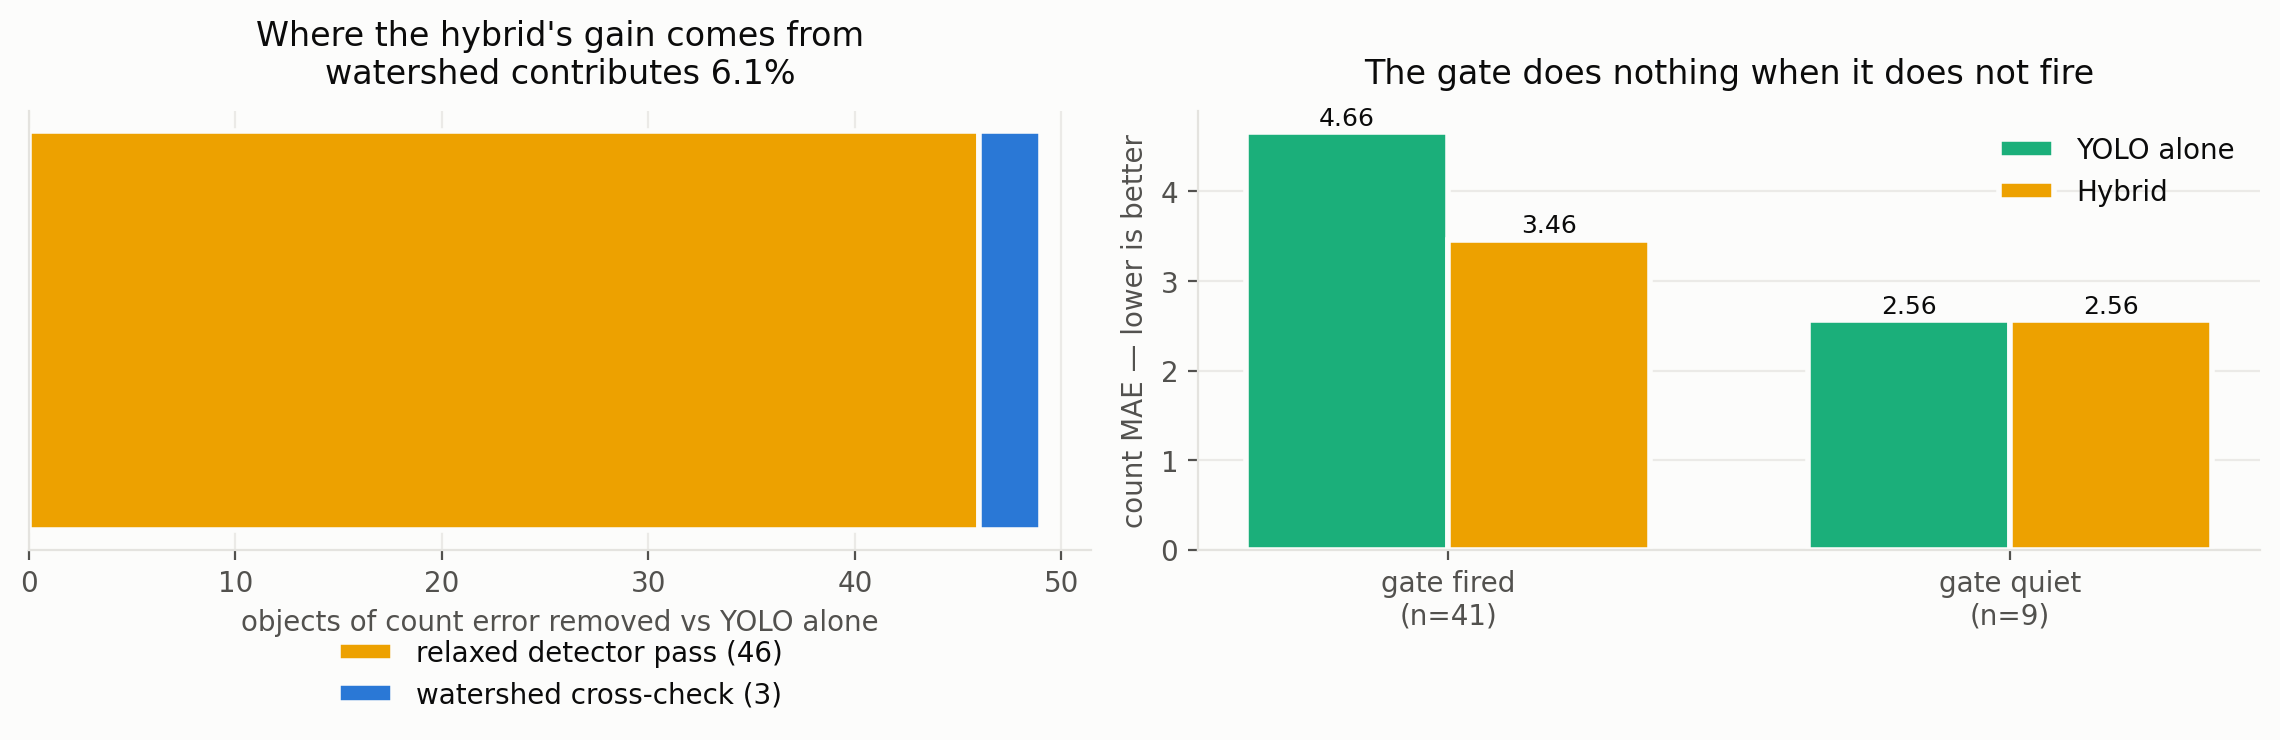
\includegraphics[width=0.95\textwidth]{ablation_attribution.png}
\caption{Phase~3 hybrid architecture: YOLOv8 backbone with confidence-routed
Watershed refinement and density-aware fusion.}
\label{fig:archp3}
\end{figure}

The system operates in five stages:
\begin{enumerate}
    \item \textbf{Normal detection}: Run YOLOv8 at confidence threshold
          $\tau_n = 0.25$ with NMS IoU threshold $\theta_n = 0.45$.
    \item \textbf{Density estimation}: Compute edge density using Canny
          edge detection:
          \begin{equation}
          \rho = \frac{\sum_{x,y} \mathbf{1}[E(x,y) > 0]}{H \times W}
          \label{eq:density}
          \end{equation}
          where $E$ is the Canny edge map.
    \item \textbf{Dense mode trigger}: If $\rho > 0.08$ or
          $\text{count}_{\text{normal}} \geq 12$, activate dense mode.
    \item \textbf{Dense re-detection}: Re-run YOLOv8 at lower threshold
          $\tau_d = 0.15$ with relaxed NMS $\theta_d = 0.35$.
    \item \textbf{Weighted fusion}: Combine predictions:
          \begin{equation}
          \hat{c} = \lfloor 0.4 \cdot c_{\text{normal}} + 0.6 \cdot c_{\text{dense}} \rfloor
          \label{eq:fusion}
          \end{equation}
\end{enumerate}

\subsection{Training Configuration}

Phase~3 training uses 800~images (2$\times$ Phase~2) with stronger
regularisation to address Phase~2 overfitting:

\begin{table}[H]
\centering
\caption{Phase~3 fine-tuning hyperparameters.}
\label{tab:hparams3}
\begin{tabular}{lll}
\toprule
\textbf{Parameter} & \textbf{Value} & \textbf{Rationale} \\
\midrule
Training images    & 800     & 2$\times$ Phase~2 to reduce overfitting \\
Epochs             & 4       & Early convergence (best at epoch 1)    \\
Batch size         & 16      & Colab T4 GPU (16~GB VRAM)              \\
Image size         & 640     & Standard YOLO input resolution         \\
Dropout            & 0.3     & 3$\times$ Phase~2 for regularisation   \\
Weight decay       & 0.001   & 2$\times$ Phase~2 L2 penalty            \\
Device             & T4 GPU  & Google Colab                            \\
\bottomrule
\end{tabular}
\end{table}

\subsection{Key Innovation: Conditional Coupling}

Unlike a sequential pipeline (run YOLO then Watershed), the hybrid system
uses \emph{conditional coupling}: the density estimator controls \emph{whether}
and \emph{how} the classical method is invoked.  In low-density scenes
(\nTest$-$\gateFired\ test images), YOLOv8 predictions are trusted directly.
In high-density scenes (\gateFired\ of \nTest), the system adaptively lowers
detection thresholds and fuses dual predictions.  This is the architectural
innovation that distinguishes Phase~3 from a na\"ive cascade.

% ── Phase 3 Results ──────────────────────────────────────────────────
% ── Results ───────────────────────────────────────────────────────────
\section{Results}
\label{sec:results}

Every number in this section comes from one evaluation run
(\texttt{src/evaluate.py}) in which all four methods were scored on the same
\nTest\ held-out test images, with the same metric definitions, in a single
process on one device.  The first version of this study reported each phase
separately and then tabulated the results together; because the phases used
different sample sizes, different training runs and different hardware, that
table described no experiment that was ever performed.

\resultsTable

\subsection{Metric definitions}

\textbf{Instance IoU} is class-agnostic and computed under greedy one-to-one
matching: predicted and ground-truth masks are paired by descending IoU, each
mask used at most once, and the mean is taken over \emph{ground-truth}
instances so that a missed object contributes zero.  Class-agnostic scoring is
required rather than merely convenient --- Watershed and KMeans cluster pixels
and have no concept of an object category, so class-aware scoring would
measure them against a task they never attempt.

\textbf{Count accuracy} is the fraction of images for which
$|\hat{n} - n| \le \countTol$, and \textbf{MAE} is
$\frac{1}{N}\sum |\hat{n}_i - n_i|$.

\textbf{Latency} is reported as a median with an interquartile range, measured
after warm-up.  A mean is actively misleading here: in the earlier study a
single cold-start inference of 12.7~s pulled a reported mean from roughly
96~ms to 1650~ms.

\subsection{The classical baselines fail structurally}

Watershed predicts \WsPred\ objects per image on average against \gtCount\
ground truth (Table~\ref{tab:results}): it under-counts by roughly a factor of
three.  Otsu thresholding presumes a bimodal intensity histogram, i.e.\ a
foreground separable from background by brightness alone; a natural photograph
of a crowded scene has no such separation.  The distance transform then merges
touching objects into a single basin, so the method degrades precisely where
density is highest.

KMeans fails in the opposite direction and far more severely, producing
\KmPred\ regions per image --- an order of magnitude more than there are
objects --- for MAE~\KmMae\ and count accuracy of \KmAcc\%.  Colour clustering
carries no object prior: a patterned garment fragments across clusters and
each fragment becomes an instance, while a flat surface shatters on lighting
gradients.

Neither failure is a tuning problem.  Both follow from the assumptions the
methods make, which is why the gap to a learned detector is not closable by
parameter search.

\begin{figure}[H]
\centering
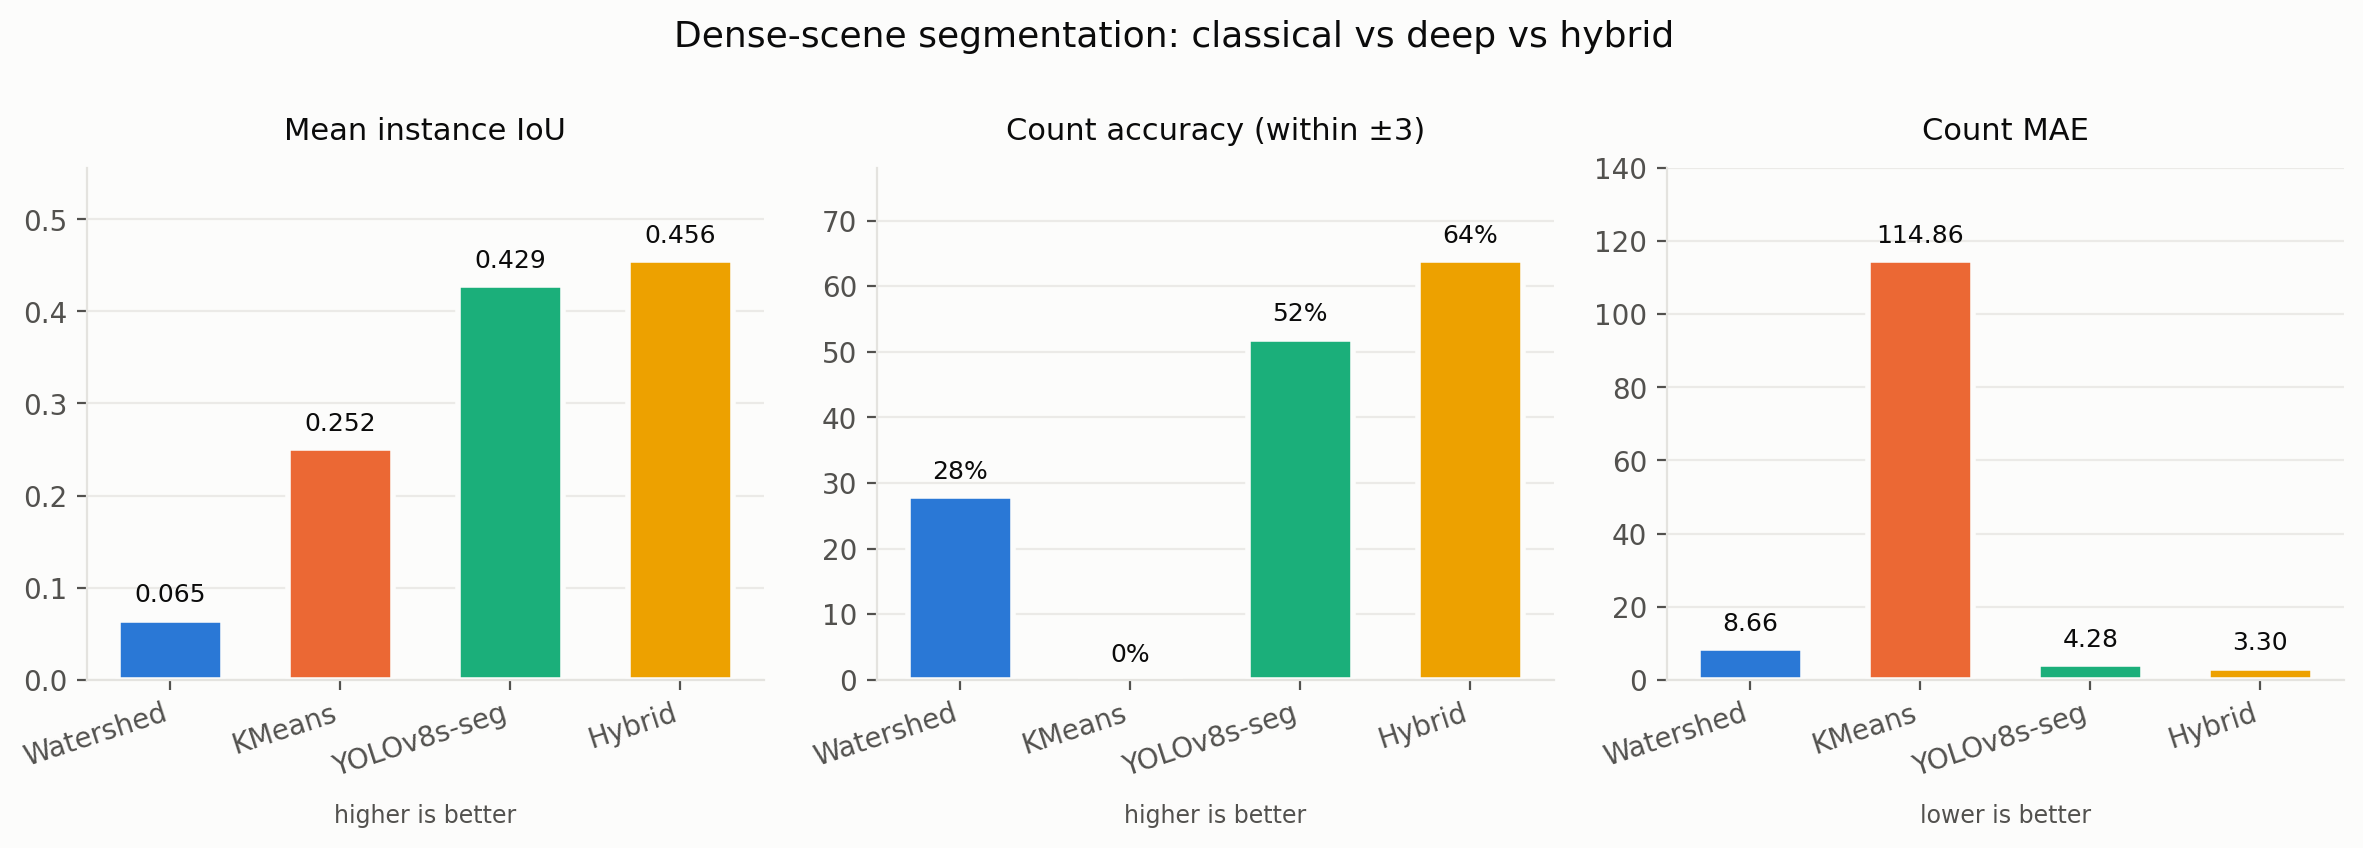
\includegraphics[width=0.95\textwidth]{comparison.png}
\caption{The three quality metrics, shown as three panels rather than one
chart with multiple axes: IoU, percentage and object-count error share no
scale, and a combined axis would imply crossings that do not exist.}
\label{fig:comparison}
\end{figure}

\subsection{Mean IoU alone is not a sufficient metric}

The KMeans row in Table~\ref{tab:results} is the most instructive result in
this study.  KMeans attains \KmIoU\ mean IoU --- comfortably above Watershed's
\WsIoU\ --- while getting the object count right on \emph{none} of the \nTest\
images.  The explanation is mechanical: emitting \KmPred\ masks against
\gtCount\ objects, greedy matching finds overlap by volume rather than by
segmenting well.

Any evaluation of dense-scene segmentation that reports overlap alone can
therefore be satisfied by over-production.  This is why counting metrics are
reported here alongside IoU for every method rather than as a secondary
diagnostic.

\begin{figure}[H]
\centering
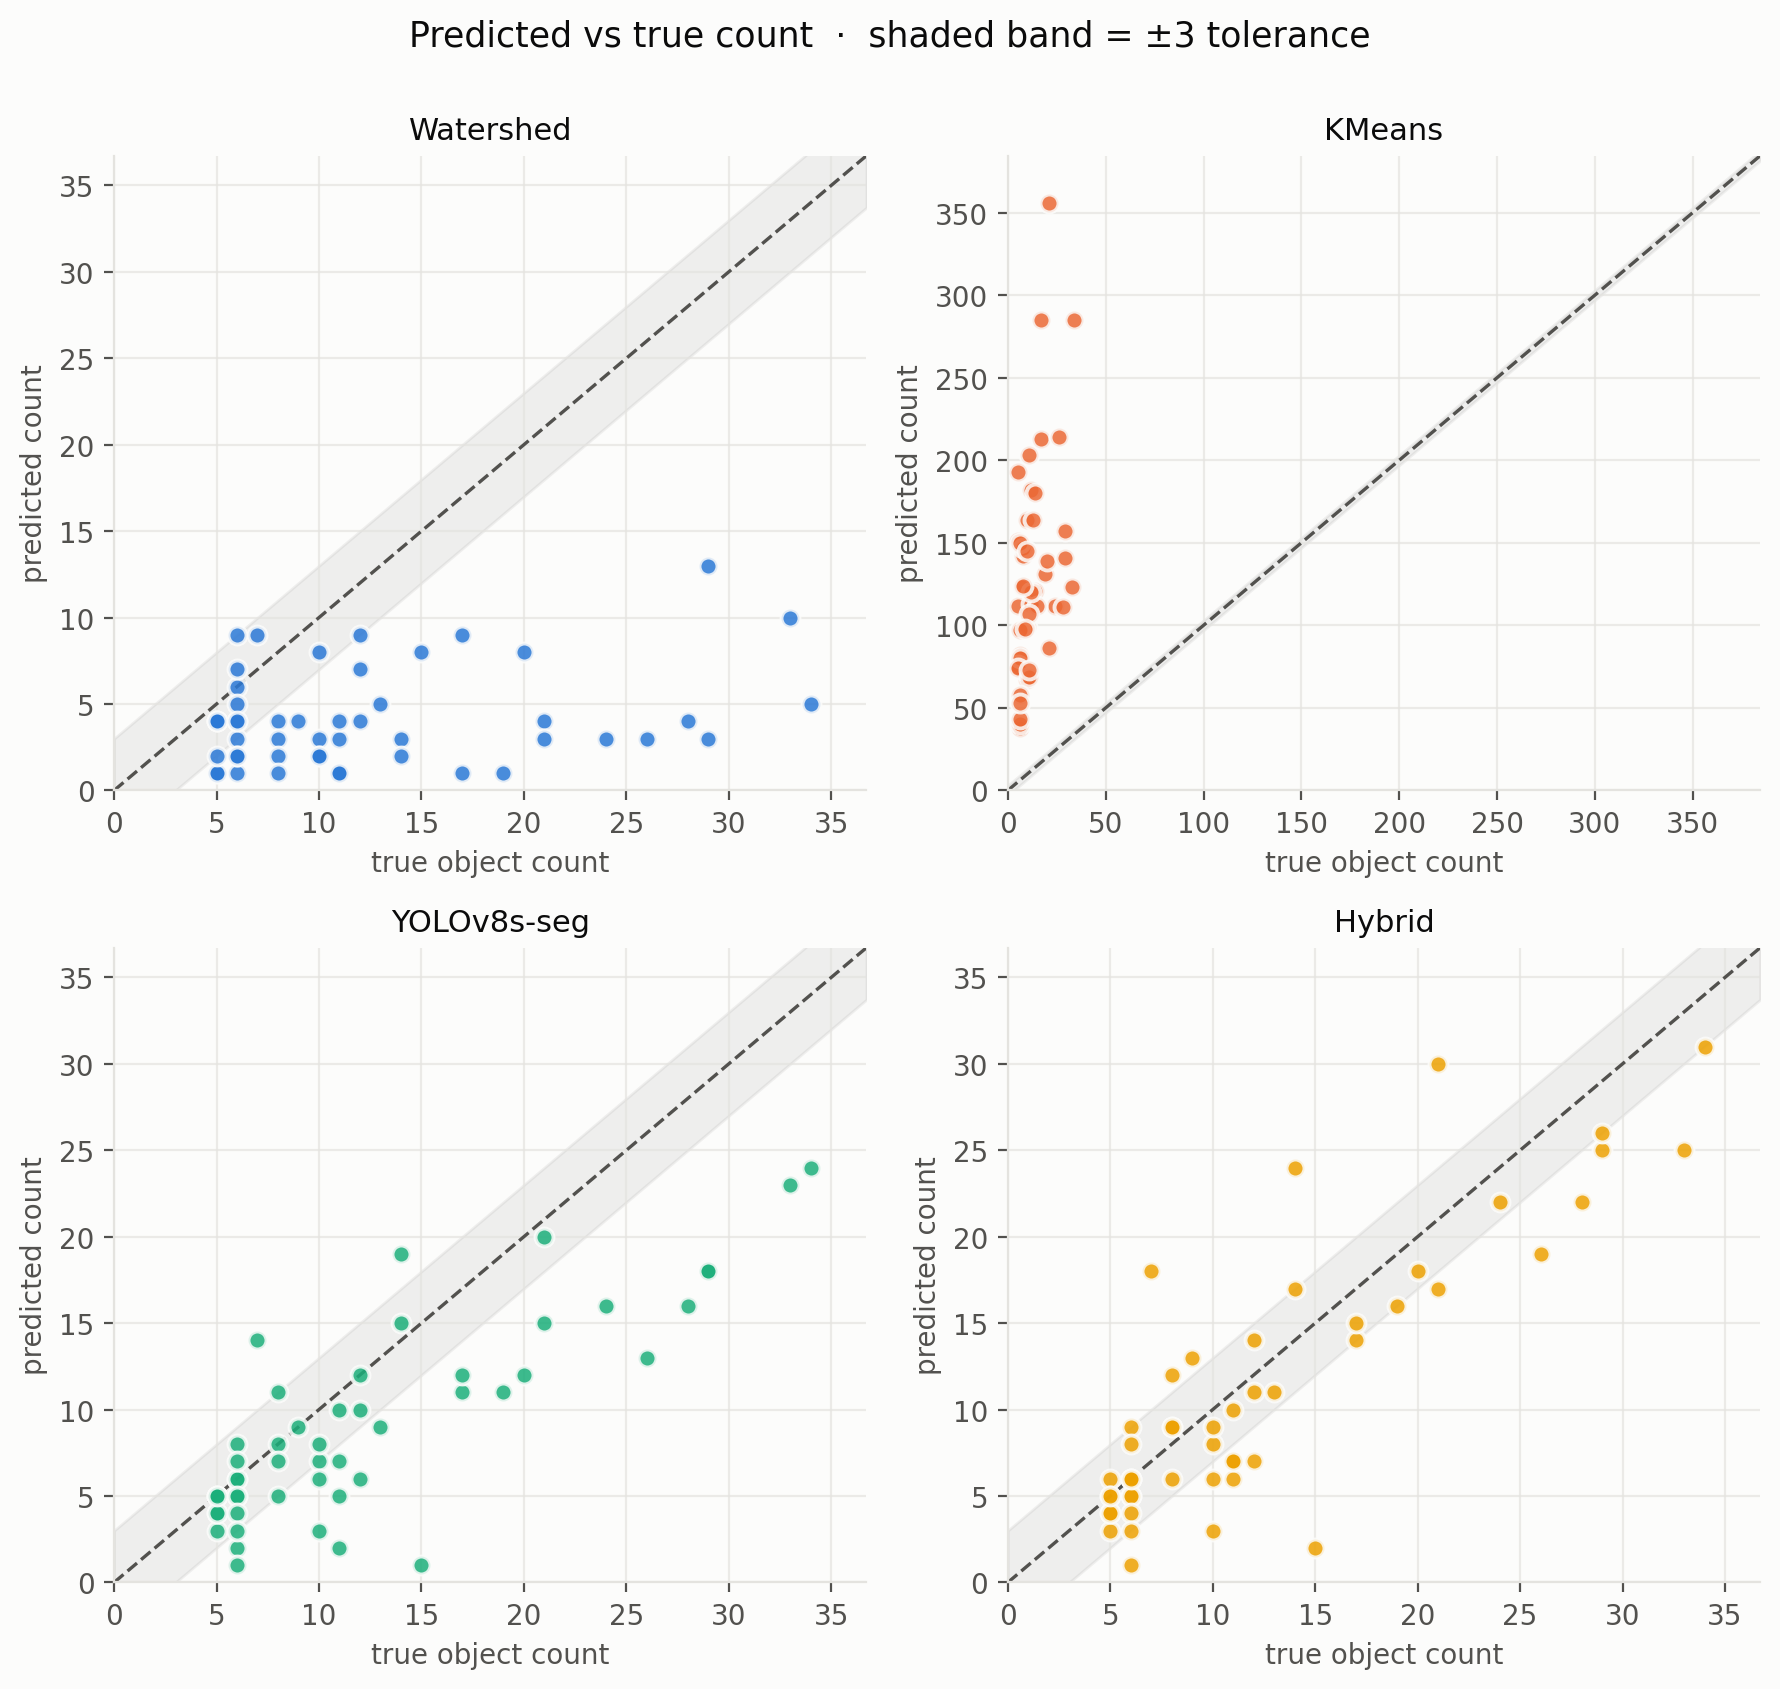
\includegraphics[width=0.90\textwidth]{count_scatter.png}
\caption{Predicted against true object count, one panel per method.  The
shaded band is the $\pm\countTol$ tolerance.  Watershed's points collapse
towards the horizontal; KMeans leaves the plotting area entirely.}
\label{fig:scatter}
\end{figure}

\subsection{Latency}

\begin{figure}[H]
\centering
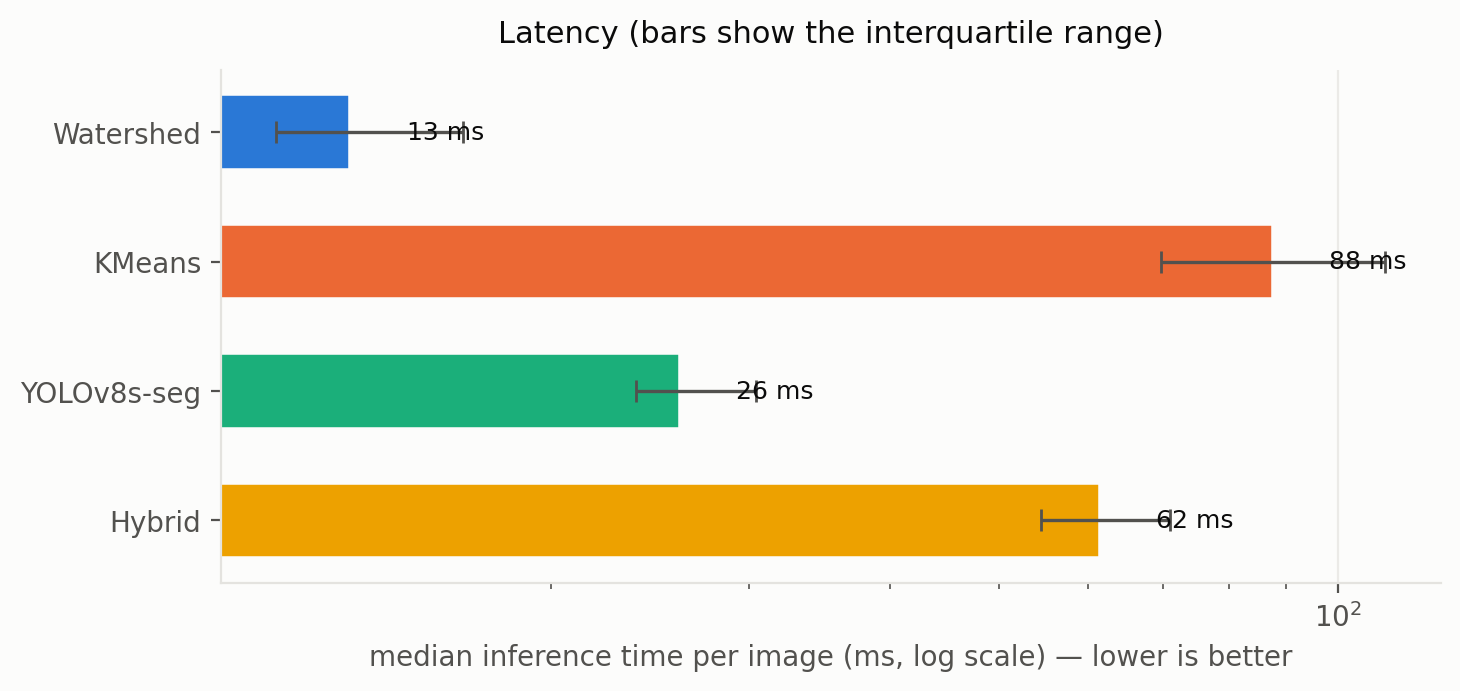
\includegraphics[width=0.85\textwidth]{inference_time.png}
\caption{Median latency per image with interquartile range, log scale.  The
deep methods run on \runDevice; the classical baselines are single-threaded
CPU.  These values compare the methods to one another and should not be
compared against published GPU timings.}
\label{fig:latency}
\end{figure}

Watershed is the cheapest method at \WsMs~ms and the least useful.  The hybrid
costs \HyMs~ms against the detector's \YoMs~ms, roughly a doubling, because a
gated second detector pass runs on most images in this dense subset.  The
Canny gate itself is negligible.

% ── Ablation ──────────────────────────────────────────────────────────
\section{Ablation: which mechanism produces the gain?}
\label{sec:ablation}

The hybrid combines two mechanisms --- a density gate that triggers a relaxed
second detector pass, and a Watershed cross-check that may raise the final
count.  Reporting only the combined result would invite the reader to assume
both contribute.  Table~\ref{tab:ablation} decomposes the improvement.

\ablationTable

Of \gainTotal\ objects of counting error removed relative to the detector
alone, \gainRelaxed\ are attributable to the relaxed detector pass and
\gainWatershed\ to the Watershed cross-check, which fires on \blendApplied\ of
\nTest\ images.  The classical component therefore accounts for
\watershedShare\% of the gain.

This is a negative result about the study's own method and it is reported as
such.  The system is more accurately described as \emph{density-aware two-pass
detection with a marginal classical correction} than as a coupling of deep and
classical paradigms in equal measure, and the title of the contribution should
follow the evidence rather than the original hypothesis.

The gate itself behaves as intended.  On the \nTest$-$\gateFired\ images where
it does not fire, the hybrid's MAE is identical to the detector's: the
mechanism costs nothing when it is not needed, which is the precondition for
its cost on the remaining \gateFired\ images being worth paying.

\begin{figure}[H]
\centering
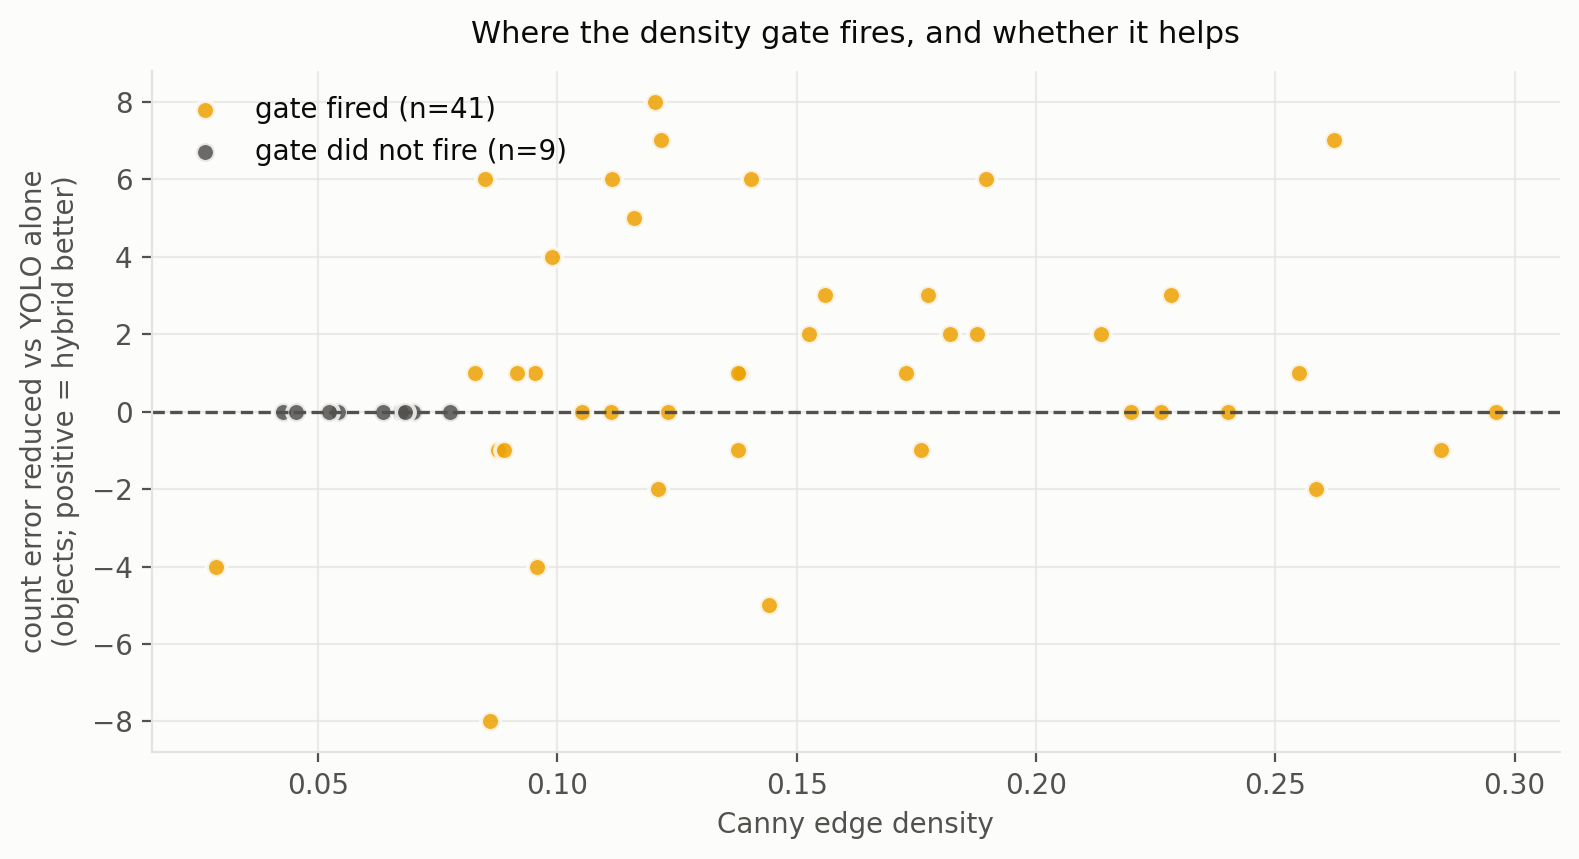
\includegraphics[width=0.90\textwidth]{density_gate.png}
\caption{Canny edge density against the counting error removed relative to
YOLOv8 alone, per test image.  Points above the dashed line are images the
hybrid improved.}
\label{fig:gate}
\end{figure}

\subsection{What this ablation does not establish}

With \blendApplied\ blend events, the Watershed cross-check is not shown to be
useless --- only that its effect is unmeasurable at this sample size.  It
improved three of those images and left the fourth unchanged.  Distinguishing
a small real effect from noise would require a substantially larger test
split, which is the clearest next step for this work.

% ── Discussion ────────────────────────────────────────────────────────
\section{Discussion}

\subsection{Why the detector handles crowding better}

A learned detector carries an object prior that neither baseline has.  Its
segmentation head predicts mask prototypes together with per-instance
coefficients, so two overlapping objects of the same class receive separate
coefficient vectors and remain distinct instances.  Watershed, working on
intensity alone, has no mechanism to keep them apart once their basins meet.

\subsection{Why relaxing the detector helps in crowds}

Non-maximum suppression removes overlapping predictions on the assumption that
overlap indicates duplication.  In a crowd that assumption is wrong: genuinely
distinct objects overlap heavily, and NMS removes real detections.  Lowering
the confidence floor and loosening the NMS threshold recovers them, at the
cost of false positives in sparse scenes --- which is exactly why the relaxed
pass is gated rather than applied everywhere.

The gate uses Canny edge density rather than the detector's own count, and the
ordering matters: if the detector has already missed the crowd, its count
cannot be the evidence that a crowd is present.

\subsection{Threats to validity}

\begin{itemize}
  \item \textbf{Sample size.}  \nTest\ test images.  The classical-versus-deep
        gap is large enough to be unambiguous; the hybrid-versus-detector gap
        should be read as a direction rather than a measured margin.
  \item \textbf{Fine-tuned on COCO, evaluated on COCO.}  The base checkpoint
        was pretrained on COCO, so this measures adaptation to a dense subset,
        not generalisation to a new domain.
  \item \textbf{Class-agnostic scoring} is necessary to place pixel-clustering
        baselines on the same scale as a detector, but it means a correct mask
        carrying the wrong label scores as a hit.
  \item \textbf{Single-polygon conversion.}  COCO instances annotated as
        several disjoint polygons retain only their largest component, a
        constraint of the YOLO segmentation label format.
  \item \textbf{Hyperparameters were not tuned on a held-out set.}  The gate
        thresholds are chosen values, not optimised ones.
\end{itemize}

% ── Conclusion ────────────────────────────────────────────────────────
\section{Conclusion}

On COCO val2017 images containing 5--50 objects, classical segmentation fails
structurally rather than marginally: Watershed under-counts by roughly
threefold (MAE~\WsMae) and KMeans over-counts by an order of magnitude
(MAE~\KmMae).  A YOLOv8s-seg model fine-tuned for \trainEpochs\ epochs reaches
\YoAcc\% count accuracy at \YoIoU\ mean IoU.  Gating a relaxed second detector
pass on Canny edge density raises this to \HyAcc\% and lowers MAE by
\maeDrop\%, at roughly double the latency.

Two findings are worth carrying forward beyond the headline numbers.  First,
mean IoU is not a sufficient metric for this task: a method emitting ten times
too many regions scored \KmIoU\ IoU while never once counting correctly.
Second, an ablation of our own method attributes \watershedShare\% of its
improvement to its classical component, which does not support describing it
as a deep-plus-classical hybrid in equal parts.

The experiment is reproducible end to end from a single seeded configuration,
and every table and figure in this report is generated from one results file
rather than transcribed.  That property, rather than any individual number, is
what the revision of this study was principally intended to establish.
% ── 13. References ────────────────────────────────────────────────────
\newpage
\printbibliography

\end{document}
